\section{Лекция 1}
\section{XII. Стационарная теория возмущений}

\subsection{\S XII.1. Резольвента и оператор Грина стационарного уравнения Шредингера}

Рассмотрим стационарное уравнение Шредингера:
\[
\hat{H}\ket{\psi} = E\ket{\psi}
\]
Перепишем его следующим образом 
\[
(\hat{1}E - \hat{H})\ket{\psi} = 0
\]

\begin{definition}
	Введём комплексную переменную $z$ и оператор $\hat{G}(z) = (\hat{1}z - \hat{H})^{-1}$ ---
	\textbf{резольвента стационарного уравнения Шредингера}.
\end{definition}

\begin{definition}
	Пусть $z = E(\in \mathbb{R})$. \textbf{Оператором Грина} стационарного УШ называется \[
	\hat{G}(E) = (\hat{z}E - \hat{H})^{-1}
	\]
\end{definition}

Замечание: 
\[
(\hat{1}E - \hat{H})\,\hat{G}(E) = \hat{1}
\]

Пусть у $\hat{H}$ есть дискретный и непрерывный спектры: $E_n$ с $\ket{E_n}$, $\braket{E_n}{E_{n'}} = \delta_{nn'}$; $E$ c $\ket{E}$, $\braket{E}{E'} = \delta(E - E')$; $\braket{E}{E_n} = 0$.

Условие полноты:
\[
\hat{1} = \sum_n \ket{E_n}\bra{E_n} + \int d\Gamma_E \ket{E}\bra{E},
\]
где $d \Gamma_E$ --- число состояний в интервале энергии $[E,\, E + dE]$.

Сделаем замену: $d \Gamma_E = \dfrac{d \Gamma_E}{dE}\,dE = \rho(E)dE$, $\rho(E)$ --- плотность состояний. Тогда, т.к. $E$ и $E_n$ --- собственные векторы $\hat{1}$ и $\hat{H}$, а значит и резольвенты, то:
\[
\hat{G}(z) = \hat{G}(z)\,\hat{1} = (\hat{1}z - \hat{H})^{-1}
\left(\sum_n \ket{E_n}\bra{E_n} + \int d \Gamma_{E'} \ket{E'}\bra{E'}\right)
= 
\]
\[
 = \sum_n \dfrac{\ket{E_n}\bra{E_n}}{z - E_n}
+ \underbrace{\int d \Gamma_{E'} \dfrac{\ket{E'}\bra{E'}}{z - E'}}_{\text{интеграл в смысле главного значения}}
\]

\begin{proposition}
	
	Полюса $\hat{G}(z)$ совпадают с $E_n$, а в непрерывном спектре --- непрерывный разрез из полюсов (см. рис.).
	
	\begin{figure}[H]
		\centering
		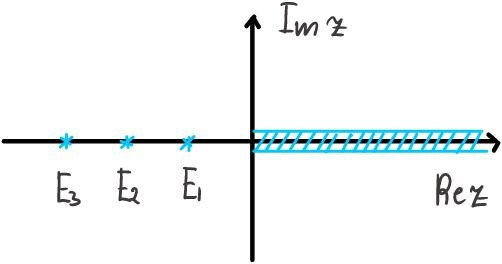
\includegraphics[width=0.75\linewidth]{images/l1_1.jpg}
	\end{figure}
	
\end{proposition}

\begin{definition}
	$\hat{G}(E)$ --- значение $\hat{G}(z)$ на одном из берегов разреза.
\end{definition}

Возьмём интеграл в смысле главного значения:
\[
\mathrm{vp}\int d \Gamma_{E'} \dfrac{\ket{E'}\bra{E'}}{z - E'}
= \int d \Gamma_{E'} \dfrac{\ket{E'}\bra{E'}}{z - E' \pm i\varepsilon} \pm i\pi \int d \Gamma_{E'} \delta(E - E')\ket{E'}\bra{E'} = 
\]
пусть $z = E$:
\[
= \int d \Gamma_{E'} \dfrac{\ket{E'}\bra{E'}}{E - E' \pm i\varepsilon}
\pm \underbrace{i\pi\rho(E)\ket{E}\bra{E}}_{\text{ = 0 как вероятность попасть в 1 точку непрерывного спектра}}
\]

Теперь можно записать:
\[
\hat{G}(E) = \sum_n \dfrac{\ket{E_n}\bra{E_n}}{E - E_n}
+ \int d \Gamma_{E'} \dfrac{\ket{E'}\bra{E'}}{E - E' \pm i\varepsilon}
\]

\begin{figure}[H]
	\centering
	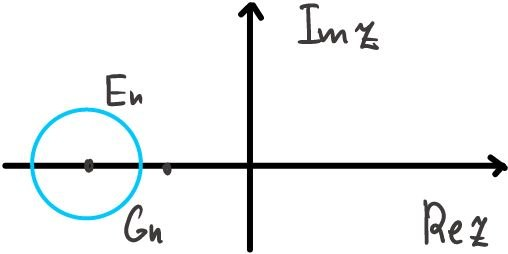
\includegraphics[width=0.55\linewidth]{images/l1_2.jpg}
\end{figure}

Найдём вычет:
\[
\oint_{G_n} \dfrac{f(z)}{z - E_n}\,dz = 2\pi i\,f(E_n)
\]

Вычет в $E_n$ --- это проектор на состояние $E_n$.



\subsection{\S XII.2. Функция Грина в координатном представлении}

\begin{definition}
	Ядро оператора Грина: $\bra{\vec{r}}\hat{G}(E)\ket{\vec{r'}} = G(E, \vec{r}, \vec{r'})$.
\end{definition}

Для стационарного уравнения Шредингера: $(\hat{1}E - \hat{H})\,\hat{G}(E) = \hat{1}$ $\Rightarrow$ берём «обкладки» $\vec{r}$:
\[
\bra{\vec{r}}(\hat{1}E - \hat{H})\hat{1}\hat{G}(E)\ket{\vec{r'}} = \delta(\vec{r} - \vec{r'})
\]
\[
\int d\vec{r''}\,\bigl(E\,\delta(\vec{r} - \vec{r'}) - \bra{\vec{r}}\hat{H}\ket{\vec{r''}}\bigr)\,G(E,\vec{r''},\vec{r'}) = \delta(\vec{r} - \vec{r'})
\]

Рассмотрим гамильтониан: $\hat{H} = \dfrac{\hat{p}^2}{2m} + U(\hat{\vec{r}})$
$\Rightarrow$ в координатном представлении $\bra{\vec{r}}\hat{H}\ket{\vec{r''}} = -\dfrac{\hbar^2}{2m}((\nabla'')^2\delta(\vec{r} - \vec{r''})) + U(\vec{r})\,\delta(\vec{r} - \vec{r''})$,
где $\nabla'' = \Bigl(\dfrac{\partial}{\partial x''}, \dfrac{\partial}{\partial y''}, \dfrac{\partial}{\partial z''}\Bigr)$, $\vec{r''} = (x'', y'', z'')$, $\Rightarrow$

\[
\left(E + \frac{\hbar^2}{2m}\,\Delta - U(\vec{r})\right) G(E, \vec{r}, \vec{r'}) = \delta(\vec{r} - \vec{r'})
\]



\subsection{\S XII.3. Функция Грина свободной частицы}

Спектр чисто непрерывен, т.е. 

\[
\hat{G}_0(E) = \int\ d \Gamma_{E'} \dfrac{\ket{E'}\times\bra{E'}}{E - E' \pm i\varepsilon}
\]

Переходим в координатное представление:
\[
G_0(E, \vec{r}, \vec{r'}) = \int d \Gamma_{E'}\dfrac{\braket{\vec{r}}{E'}\braket{E'}{\vec{r'}}}{E - E' \pm i\varepsilon}
\]

$H_0$: $\ket{rE} = \Psi_E(\vec{r})$, $\hat{H} = \dfrac{\hat{p}^2}{2m}$, $[\hat{H},\hat{p}] = 0$, $\Psi_E(\vec{r}) = A\,e^{\frac{i}{\hbar}\,\vec{p}\cdot\vec{r}}$, из $\bra{\vec{p}}\ket{\vec{p}'} = \delta(\vec{p} - \vec{p'})$ находим $A = \dfrac{1}{(2\pi\hbar)^{3/2}}$.\\

Поместим систему в ящике с бесконечно высокими стенками, очень большого объёма, тогда $\braket{\vec{p}}{\vec{p'}} = 1$ и $A = \dfrac{1}{\sqrt{V}}$.\\


А что с числом состояний $\Gamma_{E'}$? В ящике работают условия квантования $k'_x L_x = \pi u_x$ ($L_x$ --- ширина ящика); $d\Gamma_{E'} = du_x\,du_y\,d_z$; $E' = \dfrac{(\vec{p'})^2}{2m} = \dfrac{\hbar^2}{2m}(\vec{k'})^2$, где $\vec{k'} = (k'_x, k'_y, k'_z)$ $\Rightarrow$
$du_x = \dfrac{1}{2}\dfrac{L_x}{\pi} dk'_x$ (множитель $1/2$ появился, т.к. одной энергии соответствуют $+k_x$ и $-k_x$).

$d\Gamma_{E'} = du_x\,du_y\,du_z = \dfrac{1}{(2\pi)^3} L_x L_y L_z d\vec{k'} = \dfrac{V d\vec{p'}}{(2\pi\hbar)^3}$.

\begin{figure}[H]
	\centering
	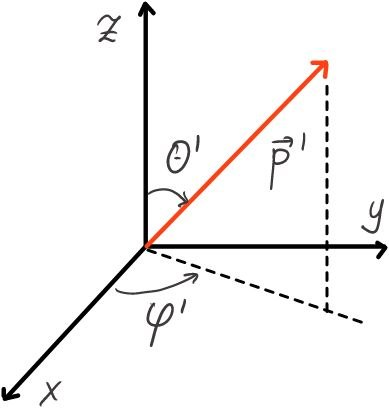
\includegraphics[width=0.3\linewidth]{images/l1_3.jpg}
\end{figure}

\begin{align*}
	d\vec{p}' &= (p')^2\,dp'\,d\Omega = \text{учтем, что } E' = \dfrac{(p')^2}{2m},\quad d\Omega = d\cos\theta'\,d\varphi' = m\,p'\,dE'\,d\Omega\\[6pt]
	G_0\!\Bigl(E = \tfrac{p^2}{2m},\,\vec{r},\,\vec{r'}\Bigr)
	&= \int d \Gamma_{E'} \dfrac{\Psi_{E'}(\vec{r})\,\Psi_E^*(\vec{r'})}{\tfrac{\vec{p}^2}{2m} - \tfrac{(p')^2}{2m} \pm i\varepsilon}
	= 2m \int \frac{d\vec{p'}\,}{(2\pi\hbar)^3}\,
	\dfrac{e^{\pm i\dfrac{\vec{p'}\cdot(\vec{r}-\vec{r'})}{{\hbar}}}}{p^2 - (p')^2 \pm i\varepsilon} = \\
	&= \text{перейдем в сферические координаты такие, что вектор }\vec{z} || (\vec{r} - \vec{r'}) = \\
	&= \dfrac{2m}{(2\pi\hbar)^3}
	\int_0^\infty \dfrac{p'\,dp'}{p^2 - (p')^2 \pm i\widetilde{\varepsilon}}
	\int_{-1}^{+1} e^{\dfrac{i}{\hbar}\,p'|\vec{r}-\vec{r'}|\cos\theta'}\,d\cos\theta'
	\int_0^{2\pi} d\varphi'\\
	&= \dfrac{m}{2 i \pi^2\hbar^2}
	\cdot \frac{1}{|\vec{r}-\vec{r'}|}
	\int_{-\infty}^\infty dp'\,\dfrac{p'\,e^{\dfrac{i}{\hbar}\,p'|\vec{r}-\vec{r'}|}}{p^2 - (p')^2 \pm i\widetilde{\varepsilon}}
\end{align*}
